\noindent This section evaluates the expected profit of each of the fault tolerance
methods discussed above under different system environment. We have identified 5
important parameters which affect the expected profit:
\begin{itemize}
\item Static power ratio $\rho$, which determines the portion of power that is unaffected by the execution speed.
\item SLA - The amount of reward, penalty and the required response times.
\item $N$ - The total number of tasks.
\item MTBF - The reliability of an individual node.
\item Workload - The size, $W$, of each individual task.
\end{itemize}



Without loss of generality, we normalize $\sigma_{max}$ to be 1, so
that all the speeds can be expressed as a fraction of maximum
speed. Accordingly, the task workload $W$ is also adjusted such that
it is equal to the amount of time (in hours) required for a single
task, preserving the ratios expressed in
\refeq{eq:tcm} and \refeq{eq:tcs}. The price of
energy is assumed to be 1 unit. We assume that $R$ in our reward model
is linearly proportional to the number of tasks $N$ and the maximal
reward for one task is 3 units, so the total reward for a job is $3
\times N$ units.  However, for the analysis we look
at the average of expenditure and income on each task by dividing the
total expenditure and income by $N$. In our basic configuration we
assume that the static power ratio is 0.5, the task size is 1 hour, the node MTBF 5 is
years, the number of tasks is $100000$, and the response time thresholds for
maximal and minimal rewards are 1.3 hours and 2.6 hours
respectively. Since the maximal power consumption is 1 unit, the
energy needed for the task with one process at maximal speed is also 1
unit. 

\subsection{Sensitivity to static power}

With various architectures and organizations, servers deployed at
different data centers will have different characteristics in terms of
power consumption. The static power ratio is used to abstract the
amount of static power consumed versus dynamic power.  

\begin{table}[!h]\small
	\caption{Speeds for different static power ratio. MTBF=5 years, N=100000, W=1 hour, $t_{R_1}$=1.3 hours, $t_{R_2}$=2.6 hours.}
	\centering
		\begin{tabular}{|c|c|c|c|}
		\hline
		$\rho$ & $\sigma_m$ & $\sigma_b$ & $\sigma_a$ \\
		\hline
		0.0 &	0.77 & 	0.65 & 	1.00 \\
		\hline 
		0.1 &	0.78 &	0.66 &	1.00 \\
		\hline
		0.2 &	0.83 &	0.66 &	1.00 \\
		\hline
		0.3	&   0.84 &	0.68 &	1.00 \\
		\hline
		0.4	&   0.85 &	0.70 &	1.00 \\
		\hline
		0.5	&   0.86 &	0.72 &	1.00 \\
		\hline
		0.6	&   0.87 &	0.73 &	1.00 \\
		\hline
		0.7	&	0.91 &	0.81 &	1.00 \\
		\hline
		0.8	& 	1.00 &	1.00 &	1.00 \\
		\hline
		0.9	&	1.00 &	1.00 &	1.00 \\
		\hline
		1.0	&	1.00 &	1.00 &	1.00 \\
		\hline
		\end{tabular}
	\label{tbl:rho}
\end{table}

\begin{figure}[!h]	
	\begin{center}
		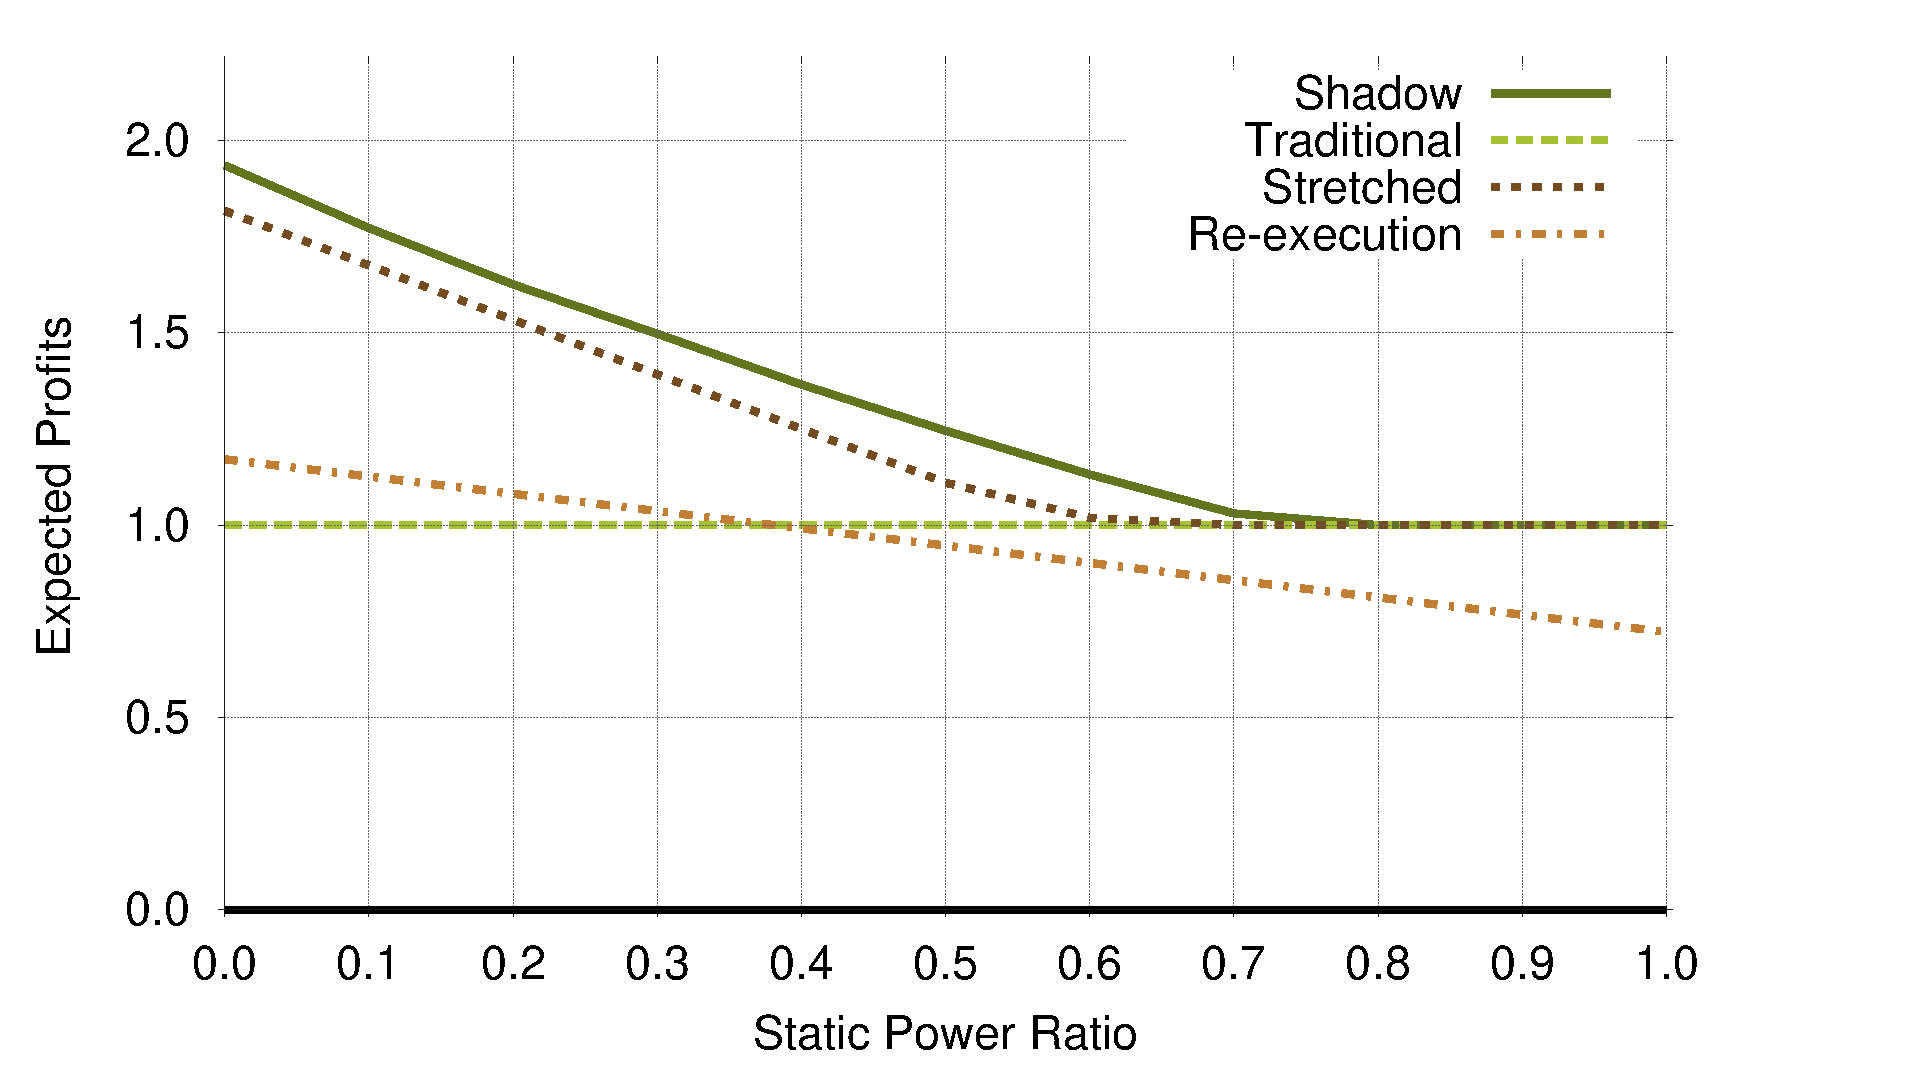
\includegraphics[width=\columnwidth]{diagrams/rho_profit.eps}
	\end{center}
	\caption{Profit for different static power ratio. MTBF=5 years, N=100000, W=1 hour, $t_{R_1}$=1.3 hours, $t_{R_2}$=2.6 hours.}
	\label{fig:rho}
\end{figure}

Table \ref{tbl:rho} shows how the profit-optimized execution speeds
of Shadow Replication will change as static power increases. The execution speeds increase to reduce the execution time as static power ration increases. Observe
that $\sigma_a$ is always equal to $\sigma_{max}$, which means that after
sensing the failure of the main process, the shadow process should always
shift to maximum speed. This is expected because the optimization will
reduce the amount of work done by the shadow process before failure
resulting in the maximum execution speed after failure, thus
minimizing the amount of repeated work. 

The potential profit gains achievable by using profit-aware
replication techniques decreases as static power increases, as is shown
in \reffig{fig:rho}. The reason is that our profit-aware
techniques rely upon the fact that one can reduce energy costs by
adjusting the execution speeds. Modern systems have a static power between 40\%-70\% and
it is reasonable to suspect that this will continue to be the case. Within
this target range of static power, Shadow Replication can achieve, on
average, 19.3\% more profit than traditional replication, 8.9\% more
than profit-aware stretched replication, and 28.8\% more than re-exeuction.


\subsection{Sensitivity to response time}

Response time is critical in the negotiation of SLA as customers
always expect their tasks to complete as soon as possible. In this
section we show a sensitivity study with respect to task response
time. We vary the first threshold $t_{R_1}$ from the minimal response
time $t_{min}$ to $1.9t_{min}$, and set the second threshold $t_{R_2}$
to be always $2t_{R_1}$. We do not show results for varying the reward
and penalty values of the SLA. The reason is that changing these
values have no effect on the choice of fault tolerance methods because
they are all affected in a similar way.

\begin{table}[!h]\small
	\caption{Speeds for different response time threshold. $\rho$=0.5, MTBF=5 years, N=100000, W=1 hour.}
	\centering
		\begin{tabular}{|c|c|c|c|}
		\hline
		$t_{R_1}$ & $\sigma_m$ & $\sigma_b$ & $\sigma_a$ \\
		\hline
		1.0	&	1.00 & 	1.00 &	1.00 \\
		\hline
		1.1	&	0.94 &	0.88 &	1.00 \\
		\hline
		1.2	&	0.89 &	0.79 &	1.00 \\
		\hline
		1.3	&	0.86 &	0.72 &	1.00 \\
		\hline
		1.4	&	1.00 &	0.00 &	1.00 \\
		\hline
		1.5	&	1.00 &	0.00 &	1.00 \\
		\hline
		1.6	&	0.84 &	0.00 &	1.00 \\
		\hline
		1.7	&	0.74 &	0.00 &	1.00 \\
		\hline
		1.8	&	0.64 &	0.00 &	1.00 \\
		\hline
		1.9	&	0.64 &	0.00 &	1.00 \\
		\hline
		\end{tabular}
	\label{tbl:t}
\end{table}

\begin{figure}[!h]	
	\begin{center}
		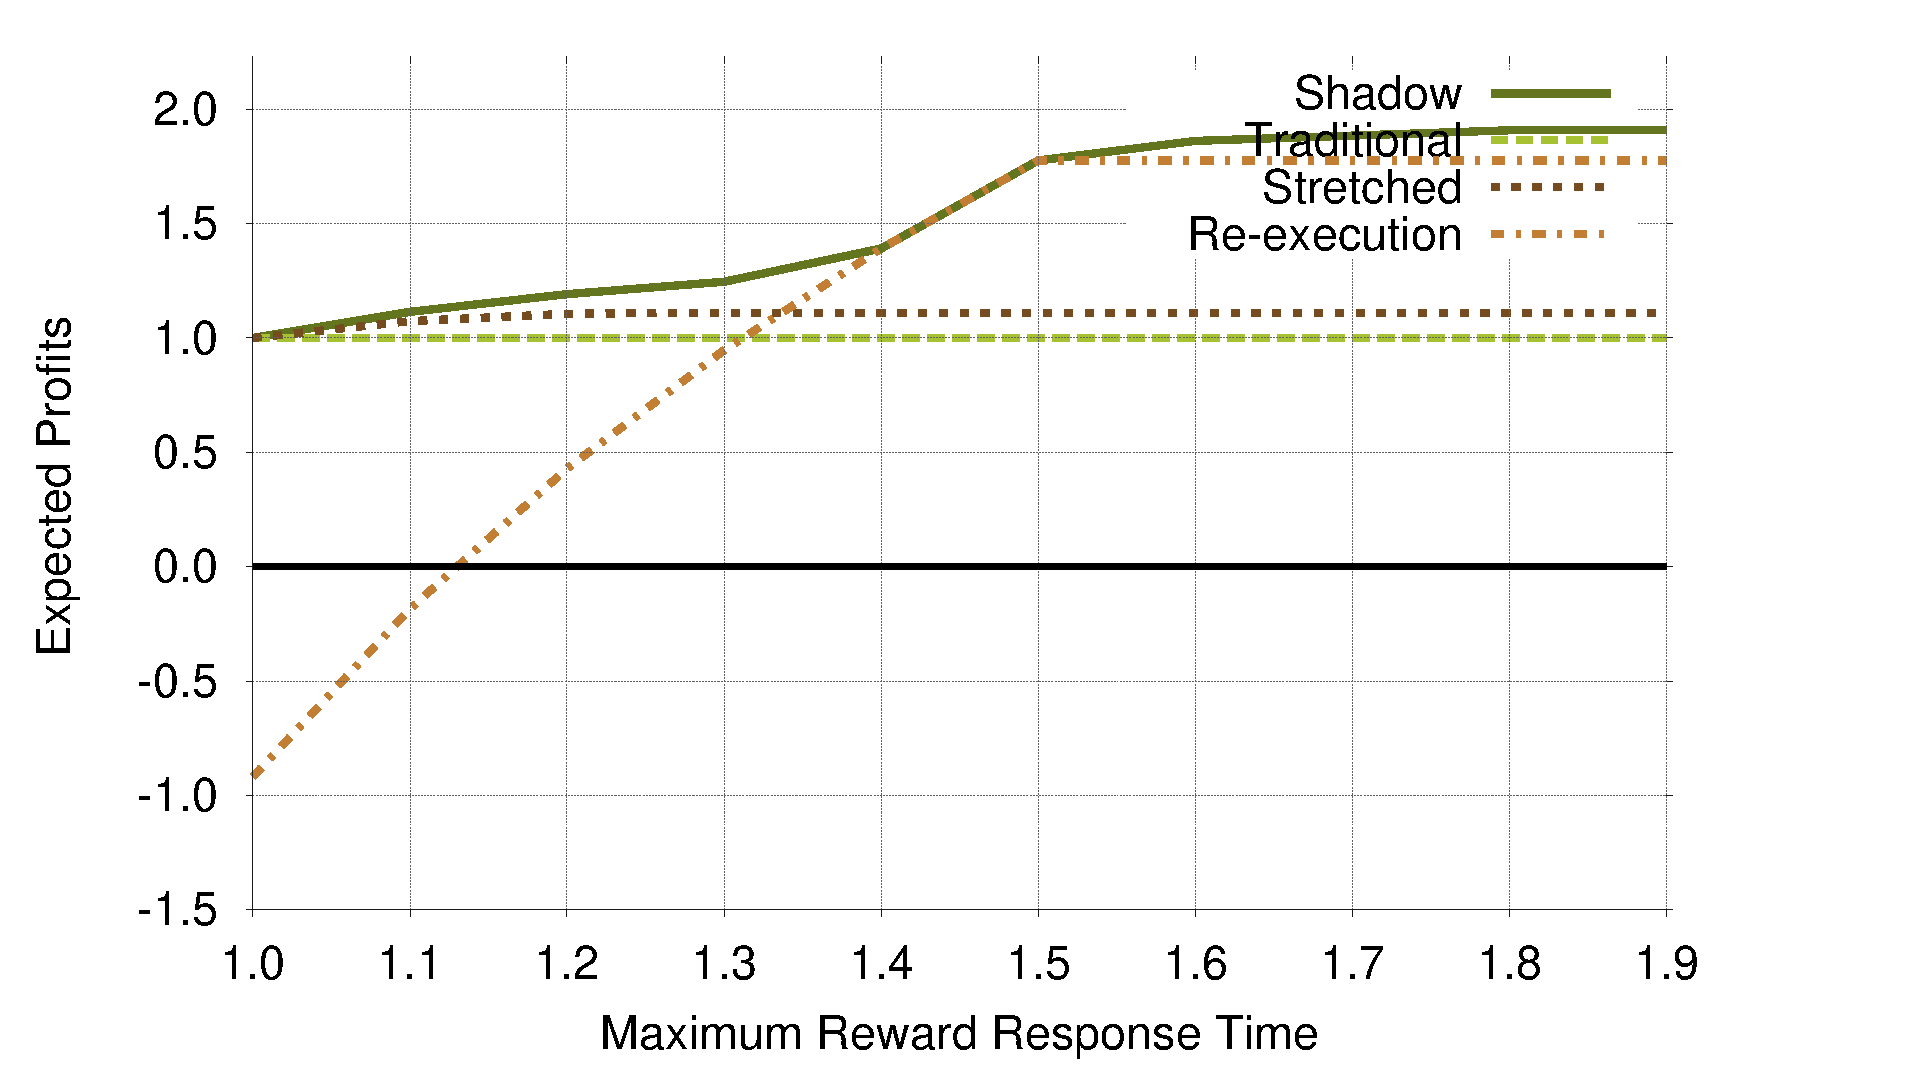
\includegraphics[width=\columnwidth]{diagrams/t_profit.eps}
	\end{center}
	\caption{Profit for different response time threshold. $\rho$=0.5, MTBF=5 years, N=100000, W=1 hour.}
	\label{fig:t}
\end{figure}

In Table~\ref{tbl:t} we see that Shadow Replication adapts the execution
speeds to take advantage of the available laxity, reducing its speeds
as laxity increases. It is clear that Shadow Replication has two different execution strategies separated by $t_{R_1}=1.4$: when time is critical, it uses both a main and a shadow from the very beginning to guarantee that task can be completed on time; when time is not critical, it mimics re-execution and starts its shadow only after a failure.
Also note that as $t_{R_1}$
approaches $t_{min}$, the speeds of the main process and the shadow process
converge, effectively causing Shadow Replication to mimic traditional
replication when faced with time-critical jobs.

\reffig{fig:t} shows the effect that targeted response time has upon
the profitability of each fault tolerance method. Compared to traditional replication, all the other methods increase their profit as the targeted
response time increases, this is expected because each of the other
techniques can make use of increased laxity in time to increase
profit. Re-execution is the most sensitive to the target response
time since it fully relies upon time redundancy, showing that it should only be used when the targeted response time is \emph{not} stringent. 
Again, Shadow Replication always achieves more profit than traditional
replication and profit-aware stretched replication, and the profit
gains are 52.8\% and 39.0\% on average. 


\subsection{Sensitivity to number of tasks}


\begin{table}[!h]\small
	\caption{Speeds for different number of tasks. $\rho$=0.5, MTBF=5 years, W=1 hour, $t_{R_1}$=1.3 hours, $t_{R_2}$=2.6 hours.}
	\centering
		\begin{tabular}{|c|c|c|c|}
		\hline
		$N$ & $\sigma_m$ & $\sigma_b$ & $\sigma_a$ \\
		\hline
		100			&	0.80	&	0.00	&	1 \\
		\hline
		1000		&	0.84	&	0.00	&	1 \\
		\hline
		10000		&	1.00	&	0.00	&	1 \\
		\hline
		100000		&	0.86	&	0.72	&	1 \\
		\hline
		1000000		&	0.86	&	0.72	&	1 \\
		\hline
		10000000	&	0.86	&	0.72	&   1 \\
		\hline
		\end{tabular}
	\label{tbl:n}
\end{table}

\begin{figure}[!h]	
	\begin{center}
			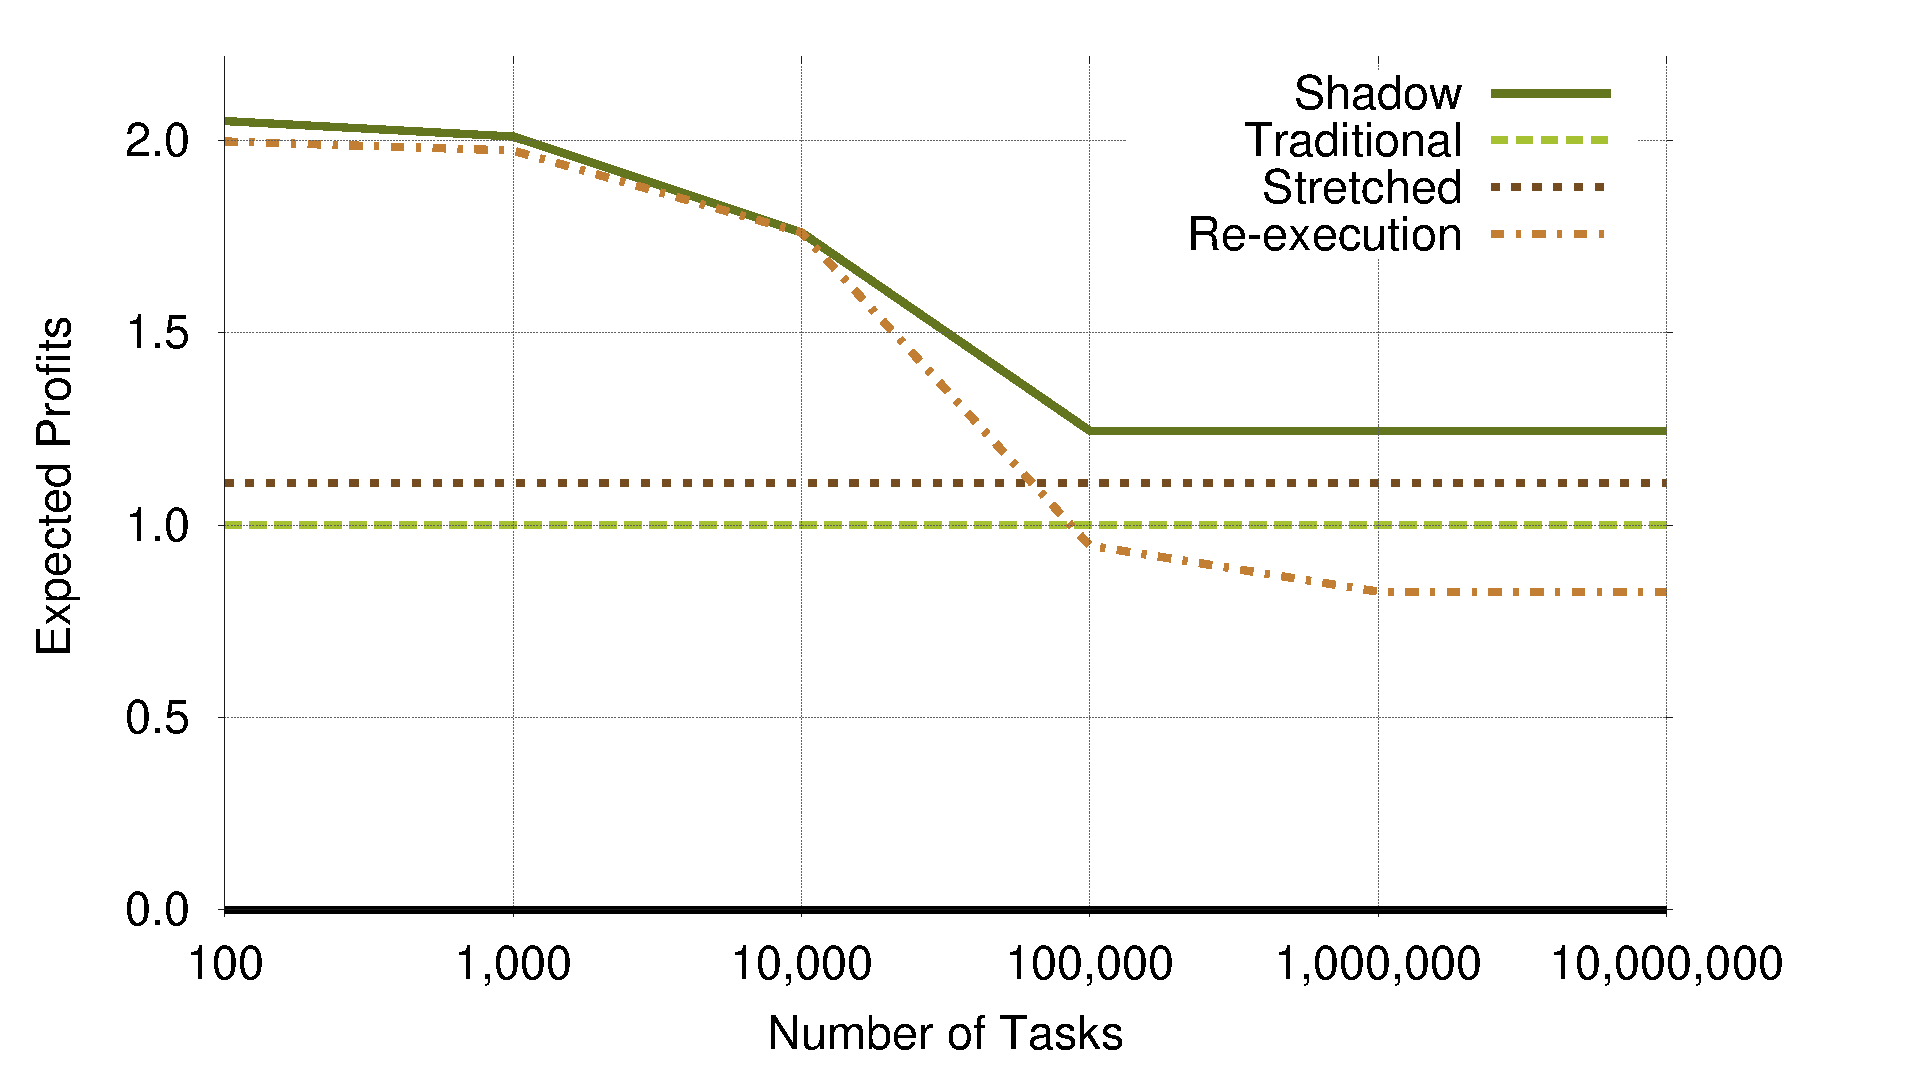
\includegraphics[width=\columnwidth]{diagrams/n_profit.eps}
	\end{center}
	\caption{Profit for different number of tasks. $\rho$=0.5, MTBF=5 years, W=1 hour, $t_{R_1}$=1.3 hours, $t_{R_2}$=2.6 hours.}
	\label{fig:n}
\end{figure}

The number of tasks has a direct influence upon the system level
failure probability because as the number of tasks increase the
probability that failure will occur to at least one task
increases. Recall that even one failure can hurt the total income
significantly, and keep the other processes waiting. Thus, shadow
replication will adjust its execution speeds to reduce the waiting
time.

Table~\ref{tbl:n} is similar to Table~\ref{tbl:t} in that there are also two execution strategies. When there are few parallel tasks, shadow
replication chooses to execute the main processes at nearly full speed and keeps
the shadow processes dormant. The
reason is that it is very likely that all main processes can finish
their tasks successfully, and the need for redundancy is thus less
significant. The other case is when there is a huge number of
tasks to execute, the shadow process would keep running at a slower speed than the main to protect the main as well as save energy. Since the system level failure probability is already 0.9 when $N$ is 100000, the speeds stay the same when $N \ge 100000$.

Figure \ref{fig:n} confirms that for small number of tasks
re-execution is more profitable than replication. However, re-execution is not scalable
as its profit decreases rapidly after N reaches 10000. At the same time, traditional
replication and profit-aware stretched replication are not
affected by the number of tasks because neither are affected by the
system level failure rate. On average, Shadow Replication achieves 43.5\%, 59.3\%, and 18.4\%
more profits than profit-aware stretched replication, traditional replication and re-exeuction, respectively. 

\subsection{Sensitivity to failure vulnerability}

The ratio between task size and node MTBF represents the tasks
vulnerability to failure, specifically it is an approximation of the
probability that failure occurs during the execution of the task. In our
analysis we found that increasing task size will have the same effect
as reducing node MTBF. Therefore, we analyze these together using the
vulnerability to failure, allowing us to analyze a wider range of
system parameters.

\begin{table}[!h]\small
	\caption{Speeds for different task size over MTBF. $\rho$=0.5, N=100000, $t_{R_1}$=1.3 hours, $t_{R_2}$=2.6 hours.}
	\centering
		\begin{tabular}{|c|c|c|c|}
		\hline
		$W/MTBF$ & $\sigma_m$ & $\sigma_b$ & $\sigma_a$ \\
		\hline
		2E-10	&	0.79 &	0.00 &	1.00 \\
		\hline
		2E-09	&	0.79 &	0.00 &	1.00 \\
		\hline
		2E-08	&	0.80 &	0.00 &	1.00 \\
		\hline
		2E-07	&	0.84 &	0.00 &	1.00 \\
		\hline
		2E-06	&	1.00 &	0.00 &	1.00 \\
		\hline
		2E-05	&	0.86 &	0.72 &	1.00 \\
		\hline
		2E-04	&	0.86 &	0.72 &	1.00 \\
		\hline
		2E-03	&	0.86 &	0.72 &	1.00 \\
		\hline
		%2E-02	&	0.86 &	0.72 &	1.00 \\
		%\hline
		\end{tabular}
	\label{tbl:mtbf}
\end{table}

\begin{figure}[!h]	
	\begin{center}
			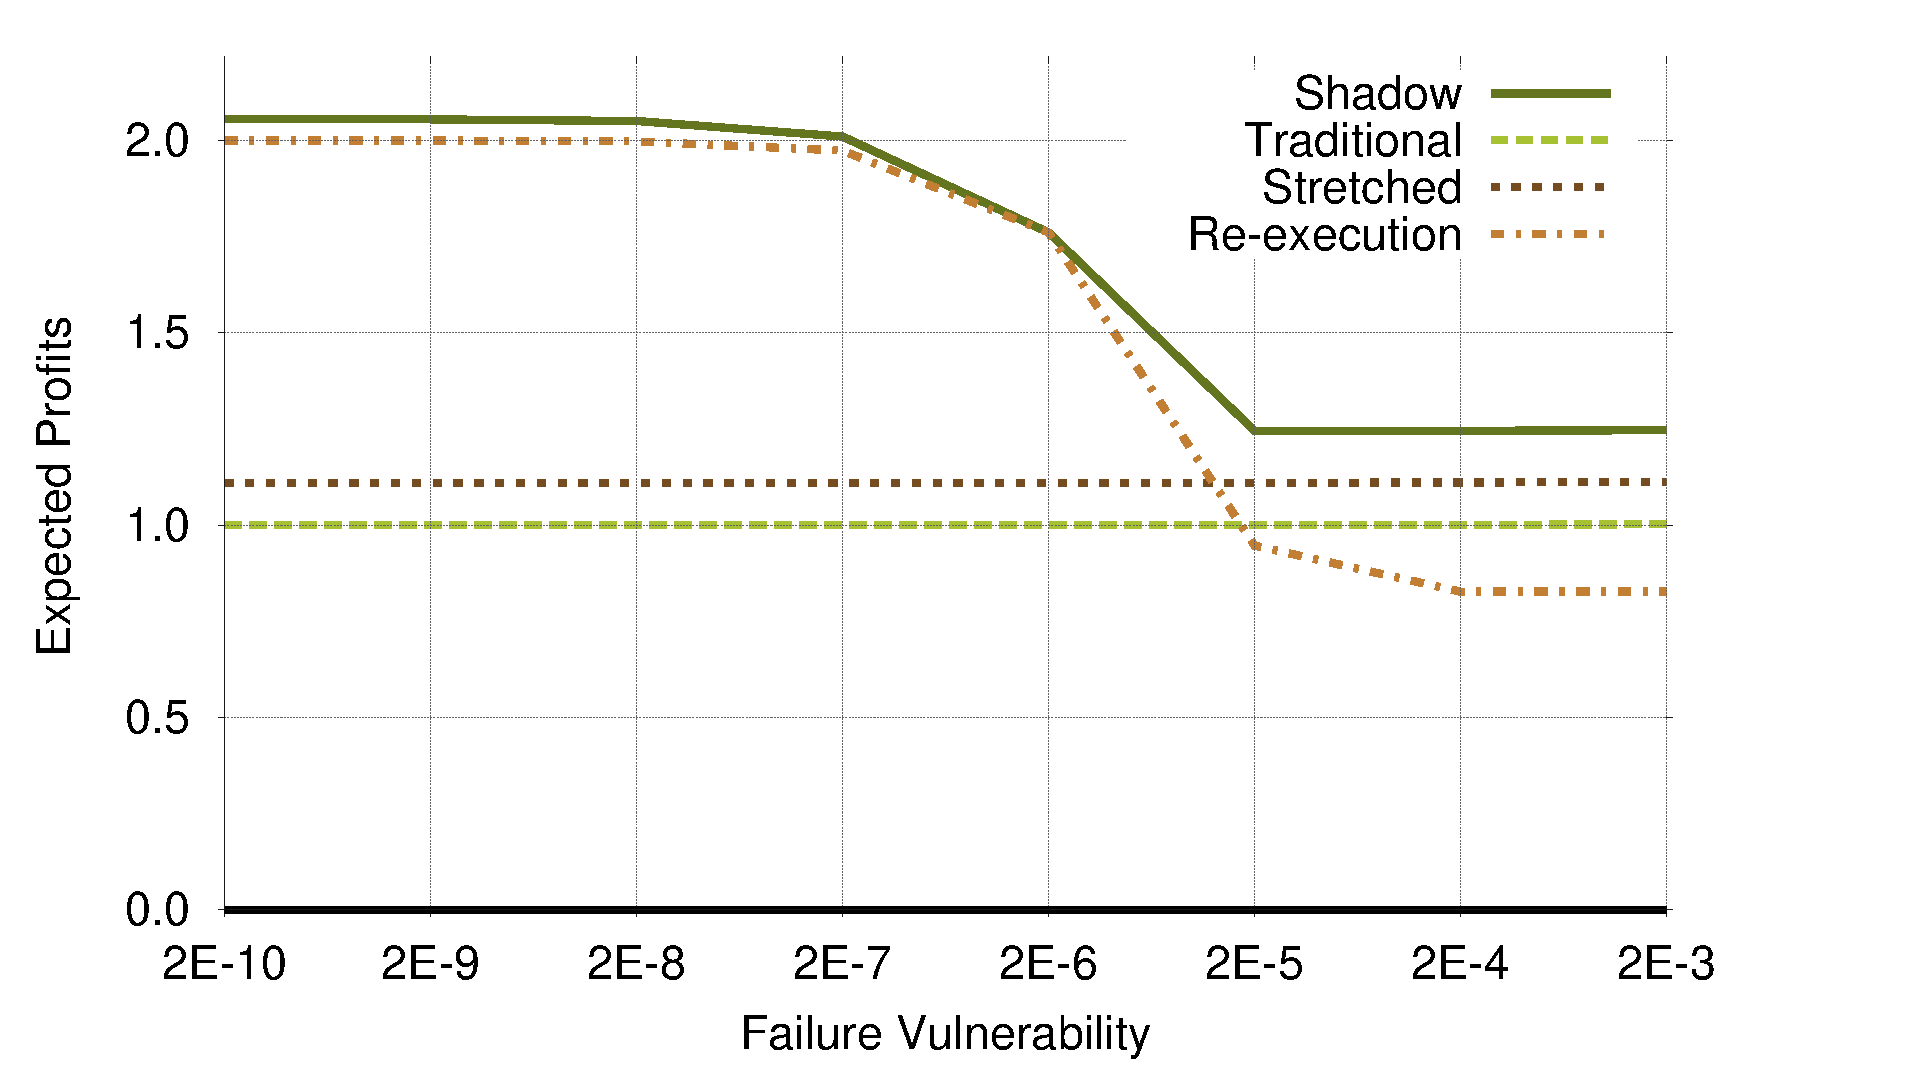
\includegraphics[width=\columnwidth]{diagrams/mtbf_profit.eps}
	\end{center}
	\caption{Profit for different task size over MTBF. $\rho$=0.5, N=100000, $t_{R_1}$=1.3 hours, $t_{R_2}$=2.6 hours.}
	\label{fig:mtbf}
\end{figure}

As seen in Table~\ref{tbl:mtbf} when the vulnerability to
failure is low the execution speeds for the shadow process is such
that no work is done before failure. However, as the
vulnerability increases, the shadow process performs more work before
failure. This is analogous to what we observed as we increased the
number of tasks (Table~\ref{tbl:n}). As expected
re-execution is desired when the vulnerability to failure is
low. As always, Shadow Replication can adjust its execution strategy to maximize the profits, as shown in Figure~\ref{fig:mtbf}.

\subsection{Application comparison}

To compare the potential benefit of ``Shadow Replication'' we evaluate
the expected profit of each resilience technique using three different
benchmark applications representing a wide range of
application~\cite{mrbs}: Business Intelligence, Bioinformatics and
Recommendation System. The business intelligence benchmark application
is a decision support system for a wholesale supplier. It emphasizes
executing business-oriented ad-hoc queries using Apache Hive. The
bioinformatics application performs DNA sequencing, allowing genome
analysis on a wide range of organisms. The recommendation system is
similar to those typically found in e-commerce sites which, based upon
browsing habits and history, recommends similar
products.

\begin{table}[h]
	\centering
		\begin{tabular}{|c|c|}
			\hline
			Application               & Processing Rate \\
			\hline
			Business Intelligence     & 3.3 (MB/s)      \\ 
			Bioinformatics            & 6.6 (MB/s)      \\ 
			Recommendation System     & 13.2 (MB/s)     \\
			\hline
                \end{tabular}
	\caption{Cloud Applications~\cite{mrbs}}
	\label{tbl:application_processing_rates}
\end{table}

Using the results of the experiments reported in \cite{mrbs}, we
derived the time required to process data for each application type (Table~\ref{tbl:application_processing_rates}). We assume that
these processing rates per task will not change when scaling the
applications to future cloud environments. This is a reasonable
assumption given that map-reduce tasks are loosely coupled and data
are widely distributed, therefore data and task workload will scale
linearly.

\begin{figure}[!h]
	
	\begin{center}
	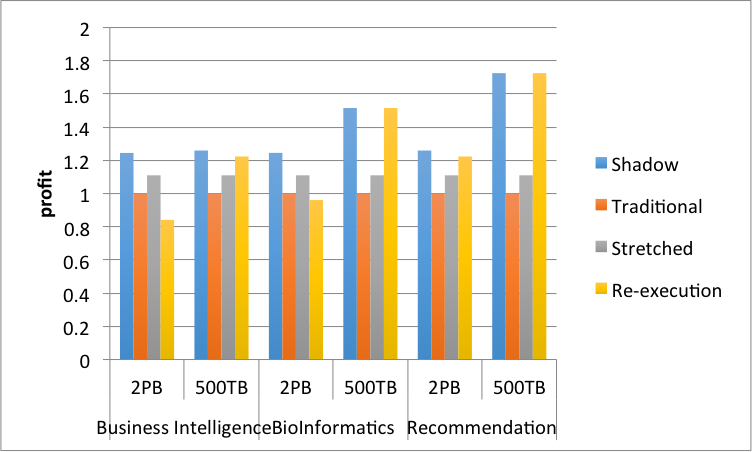
\includegraphics[width=\columnwidth]{diagrams/application_comparison.png}
	\end{center}
	\caption{Application comparison. $\rho$=0.5, N=$500000$, $t_{R_1}$=$1.3t_{min}$, $t_{R_2}$=$2.6t_{min}$.}
	\label{fig:app_compare}
\end{figure}


In Figure \ref{fig:app_compare} we compare the expected
profit for each application using each of the 4 resilience techniques. 
We consider two data sizes expected in future
cloud computing environments, 500TB and 2PB. The figure shows that
for business intelligence applications, Shadow Replication achieves significantly larger profits for both data sizes. This
is because business intelligence applications tend to be IO intensive
resulting in longer running tasks. Whereas recommendation systems tend
to require little data IO resulting in shorter running tasks making
re-execution as good as Shadow Replication. Bioinformatics tends to be in between
these two applications resulting in shadow computing performing better
when processing large datasets (2 PB) but not outstanding on smaller
datasets (500 TB). The take away from this evaluation is that for the
shown system parameters if phase execution is short, then re-execution
performs as well as Shadow Replication. Alternatively, if a phase is long (20 minutes or
greater), then Shadow Replication can be as much as 47.9\% more
profitable than re-execution. The previous sensitivity analysis can be
used to extrapolate expected profit for different system parameters.





